\subsection{Unlocking Antenna Magic: Finding the 3 dB Beamwidth!}

\begin{tcolorbox}[colback=gray!10, colframe=black, title=E9B01] What is the 3 dB beamwidth of the antenna radiation pattern shown in Figure E9-1? 
\begin{enumerate}[label=\Alph*.]
    \item 75 degrees
    \item \textbf{50 degrees}
    \item 25 degrees
    \item 30 degrees
\end{enumerate} \end{tcolorbox}

\subsubsection{Understanding 3 dB Beamwidth}

The 3 dB beamwidth of an antenna radiation pattern is defined as the angular width of the main lobe of the antenna pattern at which the power falls to half its maximum value (which corresponds to a decrease of 3 dB). It is an important specification for antennas, as it indicates how focused or wide the signal radiates into space.

To determine the 3 dB beamwidth from a given antenna radiation pattern, several aspects must be understood: 

1. \textbf{Antenna Radiation Pattern:}: This is a graphical representation of the relative strength of the radio waves emitted by the antenna in various directions. It is typically plotted in polar coordinates.

2. \textbf{Determining 3 dB Points:}: The maximum gain or power of the antenna can be identified. The 3 dB points are marked where the gain is reduced from this maximum. For many practical antenna designs, this corresponds to two specific angles from the maximum direction in which you find the same gain.

3. \textbf{Calculation of Beamwidth:}: The beamwidth can be calculated by measuring the angles to the left and right of the maximal gain direction where the gain is reduced to half that value.

\subsubsection{Calculation Example}

If we assume Figure E9-1 shows a typical antenna radiation pattern indicating maximum gain at a certain direction and the angles where the gain drops to half are 25 degrees to the left and 25 degrees to the right of the maximum gain direction, the total 3 dB beamwidth can be calculated as:

\[
\text{Beamwidth} = \theta_{\text{left}} + \theta_{\text{right}} = 25^\circ + 25^\circ = 50^\circ
\]

Therefore, the correct answer to the question is 50 degrees, which is option \textbf{B}.

\subsubsection{Figure Representation}

\begin{center}
    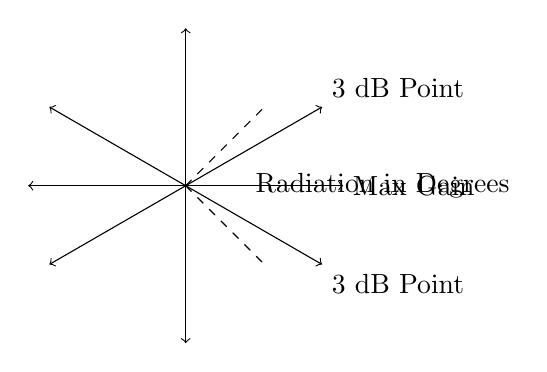
\begin{tikzpicture}
        \draw [->] (0,0) -- (2,0) node [right] {Max Gain};
        \draw [->] (0,0) -- (1.732, 1) node [above right] {3 dB Point};
        \draw [->] (0,0) -- (1.732, -1) node [below right] {3 dB Point};
        \draw [->] (0,0) -- (-2,0);
        \draw [->] (0,0) -- (0,2);
        \draw [->] (0,0) -- (0,-2);
        \draw [->] (0,0) -- (-1.732, 1);
        \draw [->] (0,0) -- (-1.732, -1);
        \draw [dashed] (0,0) -- (1,1);
        \draw [dashed] (0,0) -- (1,-1);
        \node at (2.5,0) {Radiation in Degrees};
    \end{tikzpicture}
\end{center}

In summary, the 3 dB beamwidth of 50 degrees represents how concentrated the radiation pattern of the antenna is, and by understanding the fundamental concepts outlined above, one can effectively interpret and quantify the performance of antennas in different applications.
